\begin{figure}[ht]
\begin{center}
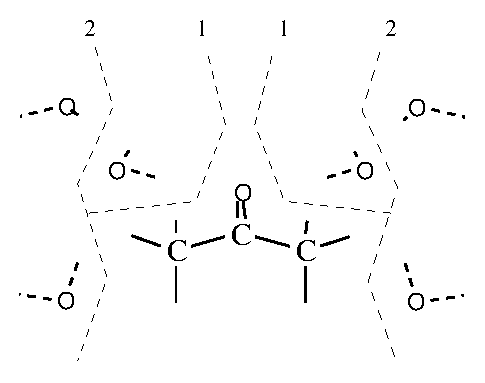
\includegraphics[width=10cm,keepaspectratio]{02_localization/images/acetone-water-frzcut-schema.eps}
\caption{\footnotesize Scheme for freeze and cut of the acetone + 6 H$_2$O
system. Surrounding water molecules have been completely frozen, and two cut
seams have been chosen to remove these molecules completely (seam ``1'') or
partially (seam ``2''). }
\label{fig:acetone-water-frzcut-schema}
\end{center}
\end{figure}
